\documentclass[../../../analisi-dei-requisiti.tex]{subfiles}

\begin{document}

\subsubsection{AUC5: Monitora organizzazione}%
\label{subs:AUC5}

\begin{figure}[H]
  \centering
  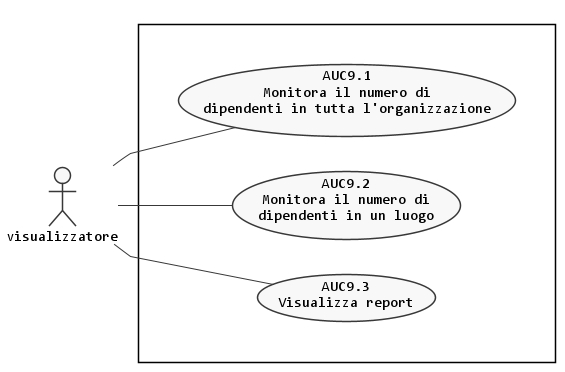
\includegraphics[width=100mm]{monitora-numero-dipendenti.png}
  \caption{AUC5: Monitoraggio organizzazione}%
  \label{fig:AUC5}
\end{figure}

\begin{description}
  \item[Codice:] AUC5;
  \item[Titolo:] Monitoraggio organizzazione;
  \item[Attori primari:] visualizzatore;
  \item[Precondizione:] il sistema deve rendere disponibile la pagina di monitoraggio dati di un'organizzazione;
  \item[Postcondizione:] il visualizzatore ottiene le informazioni di cui ha bisogno;
  \item[Scenario principale:]
  \begin{enumerate}
    \item il visualizzatore vuole ottenere delle informazioni riguardo l'organizzazione sulla quale opera.
  \end{enumerate}
\end{description}

\subsubsection{AUC5.1: Monitora il numero di dipendenti in tutta l'organizzazione}%
\label{subs:AUC5.1}
\begin{description}
  \item[Codice:] AUC5.1;
  \item[Titolo:] Monitora il numero di dipendenti in tutta l'organizzazione;
  \item[Attori primari:] visualizzatore;
  \item[Precondizione:] il sistema risponde correttamente alle interrogazioni;
  \item[Postcondizione:] il visualizzatore conosce il numero di dipendenti presenti all'interno di tutta l'organizzazione;
  \item[Scenario principale:]
  \begin{enumerate}
    \item il visualizzatore vuole sapere il numero di dipendenti presenti all'interno di tutti i luoghi dell'organizzazione.
  \end{enumerate}
\end{description}

\subsubsection{AUC5.2: Monitora il numero di dipendenti in un luogo}%
\label{subs:AUC5.2}
\begin{description}
  \item[Codice:] AUC5.2;
  \item[Titolo:] Monitora il numero di dipendenti in un luogo;
  \item[Attori primari:] visualizzatore;
  \item[Precondizione:] il sistema risponde correttamente alle interrogazioni;
  \item[Postcondizione:] il visualizzatore conosce il numero di dipendenti presenti all'interno di un luogo;
  \item[Scenario principale:]
  \begin{enumerate}
    \item il visualizzatore vuole sapere il numero di dipendenti presenti all'interno di un luogo.
  \end{enumerate}
\end{description}

\subsubsection{AUC5.3: Visualizza report}%
\label{subs:AUC5.3}
\begin{description}
  \item[Codice:] AUC5.3;
  \item[Titolo:] Visualizza report;
  \item[Attori primari:] visualizzatore;
  \item[Precondizione:] il sistema risponde correttamente alle interrogazioni;
  \item[Postcondizione:] viene stampato un report a video;
  \item[Scenario principale:]
  \begin{enumerate}
    \item si vuole visualizzare un report sotto forma tabellare, che evidenzi gli accessi, le ore trascorse all'interno dei luoghi, e quali luoghi sono più frequentati.
  \end{enumerate}
\end{description}

\end{document}
